
\chapter{The Pizza Ontology}
\label{cha:pizza-ontology}

\section{Introduction}
\label{sec:introduction}

In this section, we will create a Pizza ontology; we choose pizzas because
they are simple, well-understood and compositional (see
\href{http://robertdavidstevens.wordpress.com/2010/01/22/why-the-pizza-ontology-tutorial/}{here}
for more).

As we described in a previous Chapter~\ref{cha:an-introduction-owl},
we consider the different types of entities present in an OWL
ontology. The most (and least!) important of these are
\emph{individuals}. We say that these are the most important because
it is these individuals that are described and constrained by the
other objects. We say that they are the least important because, in
practice, many ontologies do not explicitly describe any individuals
at all.

If this seems perverse, consider a menu in a pizza shop. We might see
an item saying "Margherita\ldots{}.£5.50". The menu makes no
statements at all about an individual pizza. It is saying that any
margherita pizza produced in this resturant is going to (or already
has) cost £5.50. From the menu, we have no idea how many margherita
pizzas have been produced or have been consumed. But, menu is still
useful. The menu is comprehensive, tells you something about all the
pizzas that exist (at least in one resturant) and the different types
of pizza. This is different to the bill, which describes individuals
-- the pizzas that have actually been provided, how many pizza and how
much they all cost.  In ontological terms, the menu describes the
\textbf{classes}, the bill describes individuals \footnote{The analogy
  between a pizza menu and an ontology is not perfect. With pizza,
  people are generally happy with the classes (i.e. the menu) and
  start arguing once about the individuals (i.e. the bill); with
  ontologies it tends to be the other way around}. OWL Ontologies
built with Tawny-OWL \emph{can} describe either or both of these
entities but in most cases focus on classes.

\section{Creating the Skeleton}

As we discussed in Section~\ref{sec:creating-new-project}, it is
possible to use leiningen to create a new ontology project. We will do
this now:

\begin{verbatim}
lein new ontology take-wing-pizza
\end{verbatim}

This will create a directory called |take-wing-pizza|\footnote{The
  name of this directory is not functional important and be changed at
will}. We can now edit the files in this directory, starting with
|take/wing/pizza.clj| using either nightlight as described in
Section~\ref{sec:editing-our-ontology}, or any other IDE.


\section{Preamble}
\label{sec:preamble}

In Chapter~\ref{cha:rapid-walk-through}, we showed the standard
template for a Tawny-OWL file; and indeed, leiningen has created a
pizza themed version for us.

\begin{tawnyexample}
(ns take.wing.pizza
  (:require [tawny.owl :refer :all]))
\end{tawnyexample}

It is not absolutely critial to understand these statements, but they
are simple enough and worth explaining now, even though they will
become much more relevant and start to exploit the underlying
programming language of Tawny-OWL, that is Clojure.

Statements in Clojure are also known as ``forms''. Pretty much all
Clojure forms have the same structure; that is they are delimited by
|(| and |)|. Forms are usually named after the first letters that
appear in them, which is the name of the function they will call; so
in this case, we have a |ns| or ``namespace'' form. Forms can be
nested. The |:require| form is an example of this. In this case, the
|:require| says simply to make the Tawny-OWL functions available for
use. The colon in |:require| means that this is a
\emph{keyword}. Tawny-OWL uses these in many places to define
parameters, as we see next. Before we go any further, let's make this
slightly more complex:

\begin{tawny}
(ns take.wing.pizza
  (:require [tawny.owl :refer :all]
            [tawny.reasoner :as r]))
\end{tawny}

We will see the importance of |tawny.reasoner| later. Next, we have a
|defontology| form which looks like this:

\begin{tawnyexample}
(defontology take-wing-pizza
  :iri "http://example.com/take-wing-pizza")
\end{tawnyexample}

The name of the function |defontology| tells us something useful; as
well as creating an ontology, we are defining a name which we can use
to refer to the ontology. The name is |take-wing-pizza| which comes
next. Finally, we define some parameters -- in this case, the IRI. All
OWL ontologies require IRIs (strictly the Ontology IRI) by which they
can be refered\footnote{In Tawny-OWL, this requirement is weakened --
  if you do not put an IRI, Tawny-OWL invents one for you. This is
  okay if you are experiments, but should be changed when you publish
  an ontology.}. Here, we invent one in the |example.com| domain. You
should change this to an IRI you control. In this case, we use one
from |purl.org|.

\begin{tawny}
(defontology take-wing-pizza
  :iri "http://purl.org/ontolink/take-wing/pizza")
\end{tawny}

The semantics of this statement are quite interesting. If we had created
a new database, by default, the database would be considered to be empty
-- that is there would be no individuals in it. With an ontology, the
opposite is true. By default, we assume that there could be any number
of individuals. As of yet, we just have not said anything about these
individuals.

\section{Defining Classes}
\label{sec:defining-classes}

Next, we declare two classes. A class is a set of individuals with
shared characteristics. The basic template creates an entirely useless
|HelloWorld| task for us like so:

\begin{tawnyexample}
(defclass HelloWorld)
\end{tawnyexample}

This follows the same syntax as all forms with |(| and |)|, and
follows the convention of |defontology| -- a class object is created
as well as a name |HelloWorld| which we can use to refer to that
object. In this case, we do not add any arguments nor do we need
to. If you are using nightlight, it should look like this:

\begin{figure}
  \centering
  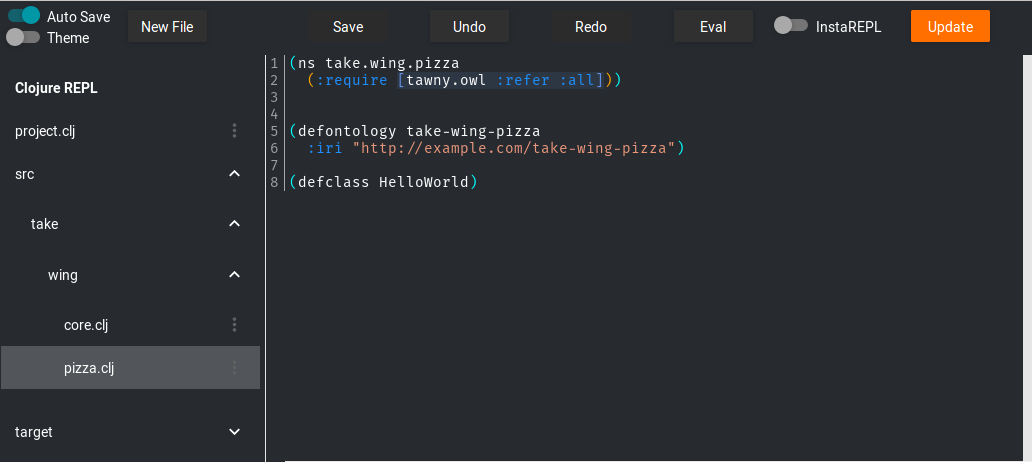
\includegraphics{images/night-pizza.png}
  \caption{A new pizza ontology}
  \label{fig:nightlight-pizza}
\end{figure}

It is possible to run, or evaluate, Tawny-OWL files as well. To see
this in nightlight, simply select ``Insta-REPL'' on the top-right.

\begin{figure}
  \centering
  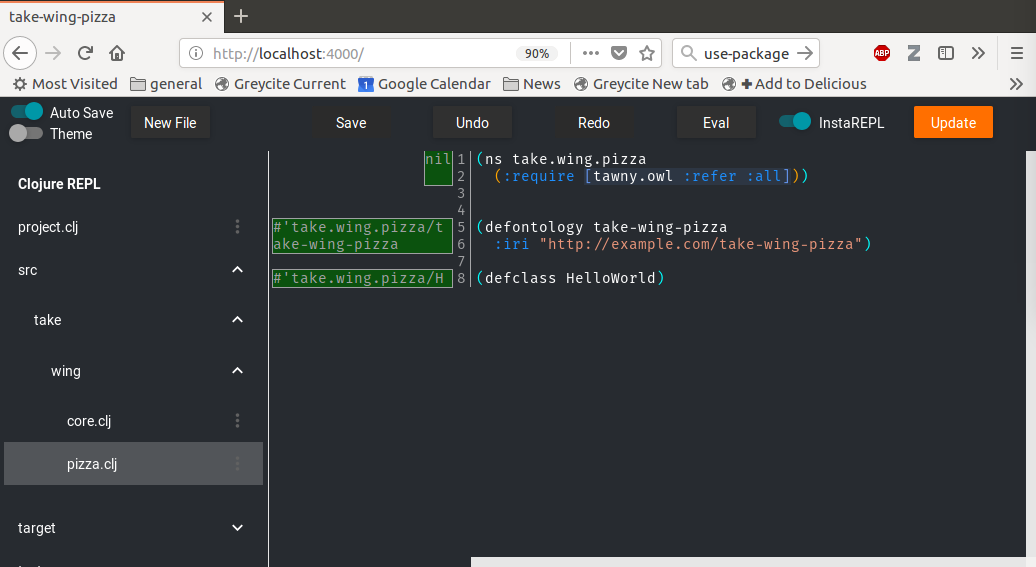
\includegraphics{images/night-instarepl.png}
  \caption{The Insta-REPL}
  \label{fig:nightlight-pizza}
\end{figure}

On the left, we can see the results of this evaluation. The actual
values are not that useful in Tawny-OWL, but the that they are green
shows that they are valid.

Clearly, as this is supposed to be an ontology of pizza rather than
classic computer programs, we will need to change this. So, first we
replace |HelloWorld| with |Pizza| and add a new class called
|PizzaComponent|.  As with our |defontology| form, have a |def| form;
however, in this case, we do not use any arguments. The semantics of
these two statements are that, there is a class called |Pizza| and
another called |PizzaComponent| which individuals may be members of.
However, we know nothing at all about the relationship between an
individual |Pizza| and an individual |PizzaComponent|\footnote{In this
  ontology, we use a naming scheme using CamelCase, upper case names
  for classes and, later, lower case properties. As with many parts of
  ontology development, opinions differ as to whether this is
  good. With Tawny-OWL it has the fortuitous advantage that it syntax
  highlights nicely, because it looks like Java class names.}.

\begin{tawnyexample}
(defclass Pizza)
(defclass PizzaComponent)
\end{tawnyexample}

To build an accurate ontology, we may wish to describe this relationship
further. We might ask the question, can an individual be both a |Pizza|
and a |PizzaComponent| at the same time. The answer to this is no, but
currently our ontology does not state this. In OWL terminology, we wish
to say that these two classes are \emph{disjoint}. We can achieve this by
adding an |as-disjoint| statement.

\begin{tawnyexample}
(as-disjoint Pizza PizzaComponent)
\end{tawnyexample}

This works well, but is a little duplicative. If we add a new class
which we wish to also be disjoint, it must be added in two places.
Instead, it is possible to do both at once. This has the advantage of
grouping the two classes together in the file, as well as semantically,
which should make the source more future-proof; should we need new
classes, we will automatically become disjoint as required.

\begin{tawny}
(as-disjoint
 (defclass Pizza)
 (defclass PizzaComponent))
\end{tawny}

If you are using Nightlight, you may find it a little hard to edit
your file to achieve this as Nightlight uses
\href{http://shaunlebron.github.io/parinfer/}{parinfer}. This puts the
parentheses in place for you. To make this statement, type
|as-disjoint| before the other two forms:

\begin{tawnyexample}
(as-disjoint)
(defclass Pizza)
(defclass PizzaComponent)
\end{tawnyexample}

Now, add two spaces in front of |(defclass Pizza)| and then |(defclass
PizzaComponent)|. The parentheses should take care of themselves.

The semantics of these statements are that our ontology may have any
number of individuals, some of which may be |Pizza|, some of which may
be |PizzaComponent|, but none of which can be both |Pizza| and
|PizzaComponent| at the same time. Before we added the |as-disjoints|
statement, we would have assumed that it was possible to be both.

As well as describing that two classes are different, we may also wish
to describe that they are closely related, or that they are
\emph{subclasses}. Where one class is a subclass of another, we are saying
that everything that is true of the superclass is also true of the
subclass. Or, in terms of individuals, that every individual of the
subclass is also an individual of the superclass.

Next, we add two more classes, in this case classes for base and
toppings. We include the statement that they have |PizzaComponent| as
a superclass. We do this by adding a |:super| argument or \emph{frame}
to our |defclass| statement.

\begin{tawnyexample}
(defclass PizzaBase
  :super PizzaComponent)
(defclass PizzaTopping
  :super PizzaComponent)
\end{tawnyexample}

In Tawny-OWL, the frames can all be read in the same way. Read
forwards, we can say |PizzaBase| has a superclass |PizzaComponent|, or
backwards |PizzaComponent| is a superclass of |PizzaBase|. Earlier, we
say the |:iri| frame for |defontology| which is read similarly --
|pizza| has the given IRI.

As every individual of, for example, |PizzaBase| is |PizzaComponent|, and no
|PizzaComponent| individual can also be a |Pizza| this also implies that no
|PizzaBase| is a |Pizza|. In otherwords, the disjointness is inherited.

As with the disjoint statement, this is little long winded; we have to name
the |PizzaComponent| superclass twice. Tawny-OWL provides a short cut for
this, with the |as-subclasses| function.

\begin{tawnyexample}
(as-subclasses
 PizzaComponent
 (defclass PizzaBase)
 (defclass PizzaTopping))
\end{tawnyexample}

We are still not complete; we asked the question previously, can you
be both a |Pizza| and a |PizzaComponent|, to which the answer is
no. We can apply the same question, and get the same answer to a
|PizzaBase| and |PizzaTopping|.  These two, therefore, should also be
disjoint. However, we can make a stronger statement still. The only
kind of |PizzaComponent| that there are either a |PizzaBase| or a
|PizzaTopping|. We say that the |PizzaComponent| class is
\emph{covered} by its two subclasses\footnote{For those from an OWL
  background, you may have noticed that ``covering'' is not part of
  the OWL standard; in fact, it's a pattern that is frequently
  used. The semantics are that \lstinline{PizzaComponent} is
  equivalent to \lstinline{PizzaBase} or \lstinline{PizzaTopping}}. We
can add both of these statements to the ontology also.

\begin{tawny}
(as-subclasses
 PizzaComponent
 :disjoint :cover
 (defclass PizzaBase)
 (defclass PizzaTopping))
\end{tawny}

We now have the basic classes that we need to describe a pizza.

\section{Properties}
\label{sec:properties}

Now, we wish to describe more about |Pizza|; in particular, we want to say
more about the relationship between |Pizza| and two |PizzaComponent| classes.
OWL provides a rich mechanism for describing relationships between individuals
and, in turn, how individuals of classes are related to each other. As well as
there being many different types of individuals, there can be many
different types of relationships. It is the relationships to other classes or
individuals that allow us to describe classes, and it is for this reason that
the different types of relationships are called \emph{properties}.

A |Pizza| is built from one or more |PizzaComponent| individuals; we first
define two properties \footnote{Actually, two \emph{object} properties, hence
  \lstinline|defoproperty|. We can also define \emph{data} properties, which
  we will see later} to relate these two together, which we call
|hasComponent| and |isComponentOf|. The semantics of this statement is to say
that we now have two properties that we can use between individuals.

\begin{tawnyhidden}
(defoproperty hasComponent)
(defoproperty isComponentOf)
\end{tawnyhidden}

As with classes, there is more that we can say about these properties. In this
case, the properties are natual opposites or inverses of each other. The
semantics of this statement is that for an individual |i| which |hasComponent|
|j|, we can say that |j| |isComponentOf| |i| also. 

\begin{tawny}
(as-inverse
 (defoproperty hasComponent)
 (defoproperty isComponentOf))
\end{tawny}

The semantics here are actually between individuals, rather than
classes. This has an important consequence with the inverses. We might
make the statement that |Pizza| |hasComponent| |PizzaComponent|, but
this does not allow us to infer that |PizzaComponent| |isComponentOf|
|Pizza|. The way that we have named our classes for pizzas, this might
be unintuitive. Consider bikes instead: just because all bicycles have
wheels, we can not assume that all wheels are parts of a bike; we
\textbf{can} assume that where a bike has a wheel, that wheel is part
of a bike. This form of semantics is quite subtle, and is an example
of where statements made in OWL are saying less than most people would
assume \footnote{We will see examples of the opposite also ---
  statements which are stronger in OWL than the intuitive
  interpretation}.

We now move on to describe the relationships between |Pizza| and both of
|PizzaBase| and |PizzaTopping|. For this, we will introduce three new parts of
OWL: subproperties, domain and range constraints and property characteristics,
which we define in Tawny-OWL as follows:

\begin{tawny}
(defoproperty hasTopping
  :super hasComponent
  :range PizzaTopping
  :domain Pizza)

(defoproperty hasBase
  :super hasComponent
  :characteristic :functional
  :range PizzaBase
  :domain Pizza)
\end{tawny}

First, we consider sub-properties, which are fairly analogous to sub-classes.
For example, if two individuals |i| and |j| are related so that
|i hasTopping j|, then it is also true that |i hasComponent j|.

Domain and range constraints describe the kind of entity that be at either end
of the property. So, for example, considering |hasTopping|, we say that the
domain is |Pizza|, so only instances of |Pizza| can have a topping, while the
range is |PizzaTopping| so only instances of |PizzaTopping| can be a topping. 

Finally, we introduce a \emph{characteristic}. OWL has quite a few
different characteristics which will introduce over time; in this case
\emph{functional} means means that there can be only one of these, so
an individual has only a single base. We do not make the same
statement about toppings, so by default, OWL will assume that you can
have any number of toppings on a pizza.

\section{Populating the Ontology}
\label{sec:populating-ontology}

We now have enough expressivity to describe quite a lot about pizzas. So, we
can now set about creating a larger set of toppings for our pizzas. First, we
describe some top level categories of types of topping. As before, we use
|as-subclasses| function and state further that all of these classes are
disjoint. Here, we have not used the |:cover| option. This is deliberate,
because we cannot be sure that these classes describe all of the different
toppings we might have; there might be toppings which fall into none of these
categories\footnote{For example, we leave open the option of a pizza
  base with nutella on it; it's not clear whether this is a pizza or
  not, but if we did decide one way or another, it would be possible
  to describe this clearly and explicitly in OWL.}. 

\begin{tawny}
(as-subclasses
 PizzaTopping
 :disjoint
 (defclass CheeseTopping)
 (defclass FishTopping)
 (defclass FruitTopping)
 (defclass HerbSpiceTopping)
 (defclass MeatTopping)
 (defclass NutTopping)
 (defclass SauceTopping)
 (defclass VegetableTopping))
\end{tawny}

When defining a large number of classes at once, Tawny-OWL also offers
a shortcut, which is |declare-classes|. While this can be useful in a
few specific circumstances, these are quite limited because it does
not allow addition of any other attributes at the same time, and in
particular labels which most classes will need. It is quite useful in
tutorial document.

\begin{tawny}
(as-subclasses
 CheeseTopping
 :disjoint

 (declare-classes
  GoatsCheeseTopping
  GorgonzolaTopping
  MozzarellaTopping
  ParmesanTopping))
\end{tawny}

A similar, if slightly longer-winded, way of defining many classes at
once is |defclassn|. We use this to define vegetables.

\begin{tawny}
(as-subclasses
 VegetableTopping
 :disjoint

 (defclassn
  [PepperTopping
    :label "Pepper Topping"]
  [GarlicTopping
    :label "Garlic Topping"]
  [PetitPoisTopping]
  [AsparagusTopping]
  [TomatoTopping]
  [ChilliPepperTopping]))
\end{tawny}

We add classes describing meat.

\begin{tawny}
(as-subclasses
 MeatTopping
 :disjoint
 (defclass HamTopping)
 (defclass PepperoniTopping))
\end{tawny}

And, finally, fruit.

\begin{tawny}
(as-subclasses
 FruitTopping
 (defclass PineappleTopping))
\end{tawny}

In this case, we have only a single entity, that is
|PineappleTopping|, so we have not made this disjoint. In fact,
Tawny-OWL would treat this as an error, since having a single disjoint
class does not really make sense, and it is mostly likely it is
wrong. This does mean that we need to remember to add this |:disjoint|
statement, if another |FruitTopping| is added.

\section{Describing a Pizza}
\label{sec:describing-pizza}

And, now finally, we have the basic concepts that we need to build a pizza.
First, we start off with a generic description of a pizza; we have already
defined the class above, so we want to extend the definition rather than
create a new one. We can achieve this using the |class| function:

\begin{tawny}
(owl-class Pizza
           :super
           (owl-some hasTopping PizzaTopping)
           (owl-some hasBase PizzaBase))
\end{tawny}

This introduces several new features of Tawny-OWL:
\begin{itemize}
\item this use of |class| requires that |Pizza| already be defined. In other
words, we are extending an existing definition. If |Pizza| is not defined,
this form will crash.
\item a new function |some|
\item we create out first \emph{unnamed} classes from a class expression -- in this
case |(owl-some hasTopping PizzaTopping)|.
\end{itemize}

The semantics of the last two of these are a little complex. Like a named
class (all of those we have seen up to now), an unnamed class defines a set of
individuals, but it does so by combining other parts of the ontology. The
|owl-some| restriction describes a class of individuals with at least one
relationship of a particular type. So
|(owl-some hasTopping PizzaTopping)| describes the set of all individuals
related by the |hasTopping| relationship to at least one
|PizzaTopping|. Or alternatively, each |Pizza| must have a
|PizzaTopping|. Or, alternatively again, for each |Pizza| there must
exist one |PizzaTopping|; it is for this reason that this form of class
is also known as an \emph{existential restriction}.

We combine the two statements to say that a |Pizza| must have at least one
base and at least one topping. Actually, we earlier defined |hasBase| with the
|:functional| characteristic, so together this says that a |Pizza| must have
exactly one base.

Finally, we can build a specific pizza, and we start with one of the simplest
pizza, that is the margherita. This has two toppings, mozzarella and tomato.
The definition for this is as follows:

\begin{tawny}
(defclass MargheritaPizza
  :super
  Pizza
  (owl-some hasTopping MozzarellaTopping)
  (owl-some hasTopping TomatoTopping)
  (only hasTopping (owl-or MozzarellaTopping TomatoTopping)))
\end{tawny}

The first part of this definition is similar to |Pizza|. It says that a
|MargheritaPizza| is a |Pizza| with two toppings, mozzarella and tomato. The
second part of the definition adds two new features of Tawny-OWL:

\begin{itemize}
\item |only| a new function which returns a \emph{universal restriction}
\item |owl-or| which returns a \emph{union restriction}
\end{itemize}

The |owl-or| statement defines the set of individuals that is either
|MozzarellaTopping| or |TomatoTopping|. The |only| statement
defines the set of individuals whose toppings are either
|MozzarellaTopping| or |TomatoTopping|. One important sting in the
tail of |only| is that it does \textbf{NOT} state that these individuals
have any toppings at all. So |(only hasTopping MozzarellaTopping)| would
cover a |Pizza| with only |MozzarellaTopping|, but also many other
things, including things which are not |Pizza| at all. Logically, this
makes sense, but it is counter-intuitive \footnote{Except to logicians,
  obviously, to whom it all makes perfect sense.}.

For completeness, we also define |HawaiianPizza| \footnote{Pizza names are, sadly,
not standardized between countries or resturants, so I've picked on which is
quite widely known. Apologies to any Italian readers for this and any other
culinary disasters which this book implies really are pizza.}.

\begin{tawny}
(defclass HawaiianPizza
  :super
  Pizza
  (owl-some hasTopping MozzarellaTopping)
  (owl-some hasTopping TomatoTopping)
  (owl-some hasTopping HamTopping)
  (owl-some hasTopping PineappleTopping)
  (only hasTopping
        (owl-or MozzarellaTopping TomatoTopping HamTopping PineappleTopping)))
\end{tawny}

We can now check that this works as expected by using the |subclass?| and
|subclasses| functions at the REPL.

\begin{verbatim}
take.wing.pizza> (subclass? Pizza MargheritaPizza)
true
take.wing.pizza> (subclasses Pizza)
#{#[Class 0x74c8b756 "HawaiianPizza"@en] #[Class 0x4f1495bd "MargheritaPizza"@en]}
\end{verbatim}

\section{A simple pattern}
\label{sec:simple-pattern}

The last definition is rather unsatisfying for two reasons. Firstly, the
multiple uses of |(owl-some hasTopping)| and secondly because the toppings are
duplicated between the universal and existential restrictions. Two features of
Tawny-OWL enable us to work around these problems. 

Firstly, the |owl-some| function is \emph{variadic} and take a single property but any
number of classes. We use this feature to shorten the definition of
|AmericanPizza|. 

\begin{tawny}
(defclass AmericanPizza
  :super
  Pizza
  (owl-some hasTopping MozzarellaTopping
            TomatoTopping PepperoniTopping)
  (only hasTopping (owl-or MozzarellaTopping TomatoTopping PepperoniTopping)))
\end{tawny}

The single |owl-some| function call here expands to three existential
restrictions, each of which becomes a super class of |AmericanPizza| --
mirroring the definition of |HawaiianPizza|.

This definition, however, still leaves the duplication between the two sets of
restrictions. This pattern is frequent enough that Tawny-OWL provides special
support for it in the form of the |some-only| function, which we use to define
the next pizza.

\begin{tawny}
(defclass AmericanHotPizza
  :super
  Pizza
  (some-only hasTopping MozzarellaTopping TomatoTopping
             PepperoniTopping ChilliPepperTopping))
\end{tawny}

The |some-only| function is Tawny-OWL's implementation of the \emph{closure} axiom.
Similarly, the use of |:cover| described earlier implements the \emph{covering}
axiom. These are the only two patterns which are directly supported by the
core of Tawny-OWL (i.e. the namespace |tawny.owl|). In later sections, though,
we will see how to exploit the programmatic nature of Tawny-OWL to build
arbitrary new patterns for yourself.

\section{Defined Classes}
\label{defined}

So far all of the classes that we have written are
\emph{primitive}. This is not a statement about their complexity. It
means that as they stand, they cannot be used to infer new facts. So,
for example, we know that a individual |MargheritaPizza| will have a
|MozzarellaTopping| and a |TomatoTopping|, but given an arbitrary
pizza we cannot determine whether it is a margherita. Or, mozzarella
and tomato toppings are \emph{necessary} for a margherita, but they
are not sufficient.

Defined classes allow us to take advantage of the power of computational
reasoning. Let us try a simple example:

\begin{tawny}
(defclass VegetarianPizza
  :equivalent
  (owl-and Pizza
           (only hasTopping
                 (owl-not (owl-or MeatTopping FishTopping)))))
\end{tawny}

Here, we define a |VegetarianPizza| as a |Pizza| with only
|MeatTopping| or |FishTopping|. The two key point about this
definition is that we have marked it as |:equivalent| rather than |:super| and
that there is no stated relationship between |VegetarianPizza| and
|MargheritaPizza|. We can confirm this at the shell. 


\begin{verbatim}
(subclasses VegetarianPizza)
=> #{}
(subclass? VegetarianPizza MargheritaPizza)
=> false
\end{verbatim}

However, now let us ask the same question of a reasoner. You may
remember that earlier we added |tawny.reasoner| to our namespace
form. This now allows us to perform computational reasoning.  First,
we choose a reasoner to use (in this case HermiT); we do this by
calling the |reasoner-factory| function; this is in the
|tawny.reasoner| namespace, which we can call by the short-cut name |r|.

\begin{verbatim}
(r/reasoner-factory :hermit)
=> #object[org.semanticweb.HermiT.Reasoner$ReasonerFactory 0x7d56d721 "org.semanticweb.HermiT.Reasoner$ReasonerFactory@7d56d721"]
\end{verbatim}

Then ask the same questions of Tawny-OWL but now using the versions of
functions prefixed with an |i| (for inferred).

\begin{verbatim}
(r/isubclasses VegetarianPizza)
=> #{#[Class 0x6487d60d "MargheritaPizza"@en]}
(r/isubclass? VegetarianPizza MargheritaPizza)
=> true
\end{verbatim}

Now, we see a different result. A |MargheritaPizza| is a subclass of
|VegetarianPizza|, even those we have never stated this explicitly.
The reasoner can infer this using the following chain of logic:

\begin{itemize}
\item |MargheritaPizza| has only |MozzarellaTopping| or |TomatoTopping|
\item |MozzarellaTopping| is a |CheeseTopping|
\item |TomatoTopping| is a |VegetableTopping|
\item |CheeseTopping| is disjoint from |MeatTopping| and |FishTopping|
\item Likewise, |TomatoTopping| is not a |MeatTopping| or |FishTopping|
\item Therefore, |MargheritaPizza| has only toppings which are not
  |MeatTopping| or |FishTopping|.
\item A |VegetarianPizza| is any |Pizza| which has only toppings which are not
  |MeatTopping| or |FishTopping|.
\item So, a |MargheritaPizza| is a |VegetarianPizza|.
\end{itemize}

Even for this example, the chain of logic that we need to draw our
inference is quite long. The version of the pizza ontology presented
here is quite small, so while we can follow and reproduce this
inference easily by hand. For a larger ontology it would be a lot
harder, especially, when we start to make greater use of the
expressivity of OWL.

Many of the statements that we have made about pizza are needed to make this
inference. For example, if we had not added |:disjoint:| to the subclasses of
|PizzaTopping|, we could not make this inference; even though we would know
that, for example, a |MozzarellaTopping| was a |CheeseTopping|; by default,
the reasoner would not assume that |CheeseTopping| was not a |MeatTopping|,
since these two could overlap. There are also some statements in the ontology
that we do not use to make this inference. For example, the reasoner does not
need to know that a |MargheritaPizza| actually has a |MozzarellaTopping| (the
statement |(some hasTopping MozzarellaTopping)|, just that if the pizza has
toppings at all, they are only mozzarella or tomato. The semantics of OWL can
be subtle, but allow us to draw extremely powerful conclusions.

\section{Recap}
\label{sec:recap-1}

In this chapter, we have described:

\begin{itemize}
\item The basic syntax of Tawny-OWL
\item New ontologies are created with |defontology|
\item Ontologies consist of classes and properties
\item Classes describe a set of individuals
\item Properties describe relationships between individuals
\item Defined classes allow us to make inferences using comptutational
  reasoning.
\end{itemize}

In addition, we have introduced the following semantic statements:
\begin{itemize}
\item Subclass relationships
\item Disjoint classes
\item Covering axioms
\item Inverse properties
\item Domain and range constraints
\item Functional characteristics
\item |some| and |only| restrictions, and the |some-only| pattern
\item |or| and |not| restrictions
\end{itemize}

